\documentclass[12pt]{article}
\usepackage[english]{babel}
\usepackage[utf8x]{inputenc}
\usepackage{amsmath}
\usepackage{graphicx}
\usepackage{caption}
\usepackage{booktabs}
\usepackage{float}
\usepackage[colorinlistoftodos]{todonotes}
\usepackage{subcaption}
\usepackage[colorlinks=true, linkcolor=blue]{hyperref}
\usepackage{array}
\usepackage{makecell}
\usepackage{siunitx}
\usepackage[margin=1in]{geometry}
\usepackage[most]{tcolorbox}
\setlength{\parskip}{0.5em}
\usepackage{titlesec}
\usepackage{placeins}
\titlespacing*{\section}{0pt}{1.2ex plus 0.5ex minus 0.2ex}{0.6ex}
\titlespacing*{\subsection}{0pt}{1ex plus 0.4ex minus 0.2ex}{0.4ex}
\titlespacing*{\subsubsection}{0pt}{0.8ex plus 0.3ex minus 0.2ex}{0.3ex}
\renewcommand{\topfraction}{0.9}
\renewcommand{\bottomfraction}{0.8}
\renewcommand{\textfraction}{0.07}
\renewcommand{\floatpagefraction}{0.8}
\setcounter{topnumber}{3}
\setcounter{bottomnumber}{2}
\setcounter{totalnumber}{5}
\setlength{\parindent}{0pt}
\setlength{\textfloatsep}{10pt plus 2pt minus 2pt}
\setlength{\floatsep}{8pt plus 2pt minus 2pt}
\setlength{\intextsep}{8pt plus 2pt minus 2pt}
\newtcolorbox{samplecalc}[1]{breakable, colback=gray!5, colframe=gray!55, boxrule=0.4pt, arc=1pt,
  left=8pt, right=8pt, top=4pt, bottom=2pt, title={#1}, fonttitle=\bfseries\small,
  coltitle=black, colbacktitle=gray!20, before skip=6pt, after skip=8pt, fontupper=\small,
  before upper={\setlength{\abovedisplayskip}{1pt}\setlength{\belowdisplayskip}{1pt}\setlength{\abovedisplayshortskip}{1pt}\setlength{\belowdisplayshortskip}{1pt}\setlength{\jot}{1.5pt}}}
\graphicspath{{./}{figures/}{../figures/}}
\newcolumntype{C}[1]{>{\centering\arraybackslash}p{#1}}
\bibliographystyle{ieeetr}


\begin{document}

\begin{titlepage}

\newcommand{\HRule}{\rule{\linewidth}{0.5mm}} % Defines a new command for the horizontal lines, change thickness here

\center % Center everything on the page

%----------------------------------------------------------------------------------------
%	HEADING SECTIONS
%----------------------------------------------------------------------------------------

\textsc{\LARGE University of Michigan}\\[1.5cm] % Name of your university/college
\textsc{\Large NERS 515}\\[0.5cm] % Major heading such as course name
\textsc{\large Nuclear Measurements Laboratory}\\[0.5cm] % Minor heading such as course title

%----------------------------------------------------------------------------------------
%	TITLE SECTION
%----------------------------------------------------------------------------------------

\HRule \\[0.4cm]
{ \huge \bfseries Laboratory 6: Scintillation Detectors}\\[0.4cm] % Title of your document
\HRule \\[0.7cm]

%----------------------------------------------------------------------------------------
%	AUTHOR SECTION
%----------------------------------------------------------------------------------------

\Large \emph{Authors:}\\
Celing \textsc{Li}\\
Charalampos Alexander \textsc{Korfiatis}\\[0.7cm] % Your name

%----------------------------------------------------------------------------------------
%	DATE SECTION
%----------------------------------------------------------------------------------------

{\large \today}\\[0.7cm] % Date, change the \today to a set date if you want to be precise

%----------------------------------------------------------------------------------------
%	LOGO SECTION
%----------------------------------------------------------------------------------------


\includegraphics[width=0.4\textwidth]{michigan_seal.png}\\[1cm] % Include a department/university logo - this will require the graphicx package

%----------------------------------------------------------------------------------------

\vfill % Fill the rest of the page with whitespace

\end{titlepage}

\begingroup
  \setlength{\parskip}{0pt} % Resets spacing only inside this group
  \tableofcontents
\endgroup

\newpage

\begin{abstract}

\phantomsection
\addcontentsline{toc}{section}{Abstract}



\end{abstract}

\section{Introduction}



\section{Theory}
\label{sec:theory}

1. purpose of PMT, dynodes, coupling compounds

2. purpose of scintillators, how they work with PMTs, scintillation efficiency

\subsection{Types of Scintillators}
\label{subsec:scint_types}

\begin{itemize}
    \item \textbf{Inorganic:} crystals in which light comes from the electronic band structure of the lattice. Activator impurities such as Tl create states within the band gap where electron-hole pairs recombine and emit visible photons. Inorganic scintillators have high density, high $Z$ and high light yield, which makes them well suited to $\gamma$-ray spectroscopy. Their decay times are relatively slow, from hundreds of ns to a few $\mu$s~\cite{knoll}.

    \begin{itemize}
        \item \textbf{NaI(Tl):} the standard $\gamma$-spectroscopy scintillator, with high light yield (38,000 photons/MeV), good resolution and a 0.23~$\mu$s decay time. It is hygroscopic and must be sealed.
        \item \textbf{CsI(Tl):} denser than NaI(Tl), with a higher light yield. Its emission (540~nm) is poorly matched to bialkali PMTs, which gives a pulse height only about 0.49 that of NaI(Tl). Its decay time is slow (0.68 and 3.34~$\mu$s components).
        \item \textbf{BGO (Bi$_4$Ge$_3$O$_{12}$):} intrinsic, meaning it needs no activator. It has the highest density and $Z_{\mathrm{eff}}$ of the four, and therefore the highest photopeak efficiency. Its light yield is low (8,200 photons/MeV, with a pulse height about 0.13 that of NaI(Tl)), so its resolution is poor.
    \end{itemize}

    \item \textbf{Organic:} materials in which light comes from transitions of $\pi$-electrons within individual molecules, so they scintillate in any physical form, including plastics, liquids and crystals. They are low-$Z$ and low-density, so they detect $\gamma$-rays almost entirely through Compton scattering, and they have very fast decay times (a few ns).

    \begin{itemize}
        \item \textbf{EJ-200:} a plastic scintillator with a 2.1~ns decay time and a light output of 64\% that of anthracene. It is cheap and can be made in large sizes, which suits it to counting and timing rather than $\gamma$ spectroscopy.
    \end{itemize}
\end{itemize} \cite{knoll}

\subsection{Features of a Scintillator Pulse-Height Spectrum}
\label{subsec:spectrum_features}

Cs-137 decays to Ba-137m, which emits a 661.7~keV $\gamma$-ray or, through internal conversion, X-rays near 32~keV. The scintillation light, and therefore the pulse height, is roughly proportional to the energy deposited in the crystal. The spectrum thus shows several features rather than a single line~\cite{knoll}. Full-energy deposition, by photoabsorption alone or after Compton scattering, produces the photopeak. Its relative size grows with density and $Z_{\mathrm{eff}}$, since the photoelectric cross section scales roughly as $Z^{\text{N}}$ for $\text{N} = [4,5]$. A single Compton scatter event followed by escape forms the Compton continuum, which ends at the Compton edge:

\begin{equation}
    E_C = \frac{2E_\gamma^2}{m_ec^2 + 2E_\gamma} \approx 477~\mathrm{keV}.
    \label{eq:compton_edge}
\end{equation}

Photons backscattered from surrounding material produce a backscatter peak at $E_\gamma - E_C \approx 184$~keV. The Ba X-rays appear as a peak at low energy. Statistical fluctuations in light production and collection broaden the photopeak, and the energy resolution is

\begin{equation}
    R = \frac{\mathrm{FWHM}}{H_0},
    \label{eq:resolution}
\end{equation}

where $H_0$ is the photopeak centroid. Background spectra are scaled by the live-time ratio and subtracted. At high count rates, dead time and pulse pile-up distort the spectrum \cite{knoll}.

In this lab, the photopeak centroid was used to set the HV and amplifier gain. The centroid, $R$ and photopeak-to-Compton ratio are compared across the four scintillators against their density and $Z_{\mathrm{eff}}$ (Table~\ref{tab:scintillators}). EJ-200, being low-$Z$, shows only a Compton edge. The 1''$\times$1'' NaI(Tl) spectra with and without coupling compound show the light lost at the crystal-PMT interface. The two source distances show the effects of count rate.

\section{Equipment and Procedure}

\subsection{Equipment}

The details of all equipment used in this lab are listed in Table \ref{tab:equipment}. The scintillators used and their properties are listed in Table \ref{tab:scintillators}. Our coupling compound was the Molykote High Vacuum Grease to seal the scintillators and PMT. Our source was a Cs-137 isotope with activity 10 $\mu$Ci and date June 15, 2023. All spectra were recorded using the Ortec Maestro Multichannel Analyzer (MCA) and MAESTRO software. Figure \ref{fig:block} shows the connections between the oscilloscope, amplifier, MCA, PMT, high voltage power supply (HV), and scintillator, assembled according to \cite{labmanual}.

\begin{table}[!htbp]
    \centering\footnotesize\setlength{\tabcolsep}{3pt}
    \begin{tabular}{lccccccc}
        \toprule
        \textbf{Scintillator} & \textbf{Type} & \makecell{\textbf{Density}\\(g/cm$^3$)} & \makecell{\textbf{Highest-$Z$}\\\textbf{element}} & \makecell{\textbf{Decay time}\\($\mu$s)} & \makecell{\textbf{Light yield}\\(photons/MeV)} & \makecell{\textbf{Rel. pulse}\\\textbf{height}} & \textbf{Size} \\
        \midrule
        NaI(Tl) & Inorganic & 3.67 & I (53) & 0.23 & 38,000 & 1.00 & \makecell{2''$\times$2''\\1''$\times$1''} \\
        CsI(Tl) & Inorganic & 4.51 & Cs (55) & \makecell{0.68 (64\%)\\3.34 (36\%)} & 65,000 & 0.49 & 1''$\times$1'' \\
        BGO & Inorganic & 7.13 & Bi (83) & 0.30 & 8,200 & 0.13 & 1''$\times$1'' \\
        EJ-200$^{\dagger}$ & \makecell{Organic\\(plastic)} & 1.03 & C (6) & 0.002 & 10,000 & 0.25 & 1''$\times$1'' \\
        \bottomrule
    \end{tabular}
    \caption{Scintillators used in this lab. Properties from Table~8.3 of Knoll \cite{knoll}. The relative pulse height is for fast electrons with a bialkali PMT, normalized to NaI(Tl). $^{\dagger}$EJ-200 is not listed in Knoll, so its row gives the typical plastic scintillator NE102A from the same table.}
    \label{tab:scintillators}
\end{table}

\begin{table}[H]
    \centering
    \resizebox{0.6\columnwidth}{!}{%
    \begin{tabular}{lcc}
        \toprule
        \textbf{Purpose} & \textbf{Manufacturer} & \textbf{Model} \\
        \midrule
        Oscilloscope & Agilent Technologies & DSO6052A \\
        High Voltage Power Supply & Ortec & 556 \\
        Amplifier & Ortec & 572A \\
        Multi-Channel Analyzer & Ortec & Easy-MCA \\
        Photomultiplier tube & Ortec & 266 \\
        \bottomrule
    \end{tabular}%
    }
    \caption{List of equipment used in Laboratory 6.}
    \label{tab:equipment}
\end{table}

\begin{figure} [H]
    \centering
    \includegraphics[width=0.8\linewidth]{image_block.png}
    \caption{Set-up diagram.}
    \label{fig:block}
\end{figure}

\subsection{Experimental Procedure}
\label{subsec:proced}

For all experiments, the PMT and scintillator were enclosed in a light-tight housing. We verified that there was no light leakage by using the oscilloscope to observe any unusual pulse behavior. The LLD was 0 for all measurements.

\subsubsection{Tube Gain and Applied Voltage}
\label{subsubsec:tube_gain}

A $2 \times 2$ inch NaI(Tl) crystal was optically coupled to the PMT with coupling compound and enclosed in a light-tight housing. To determine the distance of the source from the housing, we moved the source away starting from 0 cm until distinguishable pulses were observed in the scope at 26 cm. The amplifier gain was 10 for all measurements. Varying the high voltage from 600-1300 V in increments of 50, we collected a spectra for 20-sec time intervals. We recorded the photopeak channel by selecting the photopeak as the region of interest (ROI) in MAESTRO. The amplifier output was monitored on the scope for saturation (flat top of pulse amplitudes on oscilloscope), in case the amplitudes saturated before the plateau was visible.

\subsubsection{Scintillator Pulse Height Spectra}
\label{subsubsec:pulse_height_spectra}

The HV was fixed at 850 V and the amplifier gain was set to 12.6 which was when the photopeak of Cs-137 was visible at $\sim$45\% of full scale as per the lab manual \cite{labmanual}. These settings were held constant for all subsequent crystal changes. Three measurements were then taken with each crystal: a 4-min background spectrum, a 2-min spectrum with the source in contact with the detector face (0 inch distance), and a 2-min spectrum with the source 2 inches from the detector face. All spectra were recorded in MAESTRO and saved as .SPE files for later analysis, specifically for the photopeak centroid, energy resolution, net photopeak counts, and total spectrum counts.

Following the lab manual, we repeated this measurements with the scintillators in Table \ref{tab:scintillators} with and without coupling compounds \cite{labmanual}.

\section{Data}
\label{sec:data}

Count uncertainties are $\sigma_N = \sqrt{N}$ \cite{knoll}. All count times are MAESTRO live times. The dead time is $1 - t_{\text{live}}/t_{\text{real}}$. We convert MCA channels to pulse amplitude with the calibration from our Lab 2 report, done on the same Easy-MCA with 8192 channels:
\begin{equation}
V = \frac{\text{channel} - 27.6}{765.8},
\label{eq:mcacal}
\end{equation}
with an amplitude uncertainty of 25.4~mV \cite{lab2}.

\subsection{Tube Gain and Applied Voltage}

Table~\ref{tab:hv} lists the photopeak centroid of the 2''$\times$2'' NaI(Tl) crystal at each HV, 20~s per point, amplifier gain 10 (coarse 20, fine 0.5). The centroid uncertainty is found in Section~\ref{subsec:an_hv}. The manual suggests going up to 1300~V \cite{labmanual}. We stopped at 1150~V because the photopeak channel stopped increasing above 1000~V. It stayed between channel 1623 and 1639 (2.08 to 2.10~V) from 1050 to 1150~V. We did not see flat-topped pulses on the oscilloscope.

\begin{table}[!htbp]
\centering\small
\begin{tabular}{ccc|ccc}
\toprule
\textbf{HV (V)} & \textbf{Centroid (ch)} & \textbf{Ampl. (V)} & \textbf{HV (V)} & \textbf{Centroid (ch)} & \textbf{Ampl. (V)} \\
\midrule
600 & 71.16 $\pm$ 0.05 & 0.057 & 900 & 873.92 $\pm$ 0.04 & 1.105 \\
650 & 128.98 $\pm$ 0.09 & 0.132 & 950 & 1162.02 $\pm$ 0.07 & 1.481 \\
700 & 210.89 $\pm$ 0.14 & 0.239 & 1000 & 1537.17 $\pm$ 0.11 & 1.971 \\
750 & 321.05 $\pm$ 0.17 & 0.383 & 1050 & 1622.93 $\pm$ 0.07 & 2.083 \\
800 & 464.76 $\pm$ 0.18 & 0.571 & 1100 & 1630.87 $\pm$ 0.20 & 2.094 \\
850 & 647.02 $\pm$ 0.31 & 0.809 & 1150 & 1638.71 $\pm$ 0.04 & 2.104 \\
\bottomrule
\end{tabular}
\caption{Cs-137 photopeak centroid vs HV, 2''$\times$2'' NaI(Tl), 20~s live time per point, read from the MAESTRO ROI. Amplitude from Eq.~\ref{eq:mcacal} ($\pm$0.025~V).}
\label{tab:hv}
\end{table}

\subsection{Scintillator Pulse Height Spectra}

All spectra in this section used 850~V and amplifier gain 12.6 (coarse 20, fine 0.63). Each configuration has its own 4-min background, taken with the same crystal and coupling. Table~\ref{tab:spectra} lists the gross counts and dead times. Every source spectrum has a live time of 120~s and every background 240~s. Dead time was 19 to 29\% at 0~in for every inorganic crystal and below 6\% at 2~in. Figures~\ref{fig:raw} and \ref{fig:raw2} show the raw source spectra and the backgrounds.

\begin{table}[!htbp]
\centering\footnotesize\setlength{\tabcolsep}{3pt}
\resizebox{\textwidth}{!}{%
\begin{tabular}{lc|ccc|ccc}
\toprule
 & \textbf{Background} & \multicolumn{3}{c|}{\textbf{Source at 0 in}} & \multicolumn{3}{c}{\textbf{Source at 2 in}} \\
\textbf{Crystal} & \textbf{Gross} & \textbf{Gross} & $t_{\text{real}}$ (s) & \textbf{Dead (\%)} & \textbf{Gross} & $t_{\text{real}}$ (s) & \textbf{Dead (\%)} \\
\midrule
2''$\times$2'' NaI(Tl) & 47615 $\pm$ 218 & 2076818 $\pm$ 1441 & 148 & 18.9 & 545127 $\pm$ 738 & 127 & 5.5 \\
1''$\times$1'' NaI(Tl) & 11743 $\pm$ 108 & 2545628 $\pm$ 1596 & 151 & 20.5 & 182580 $\pm$ 427 & 122 & 1.6 \\
1''$\times$1'' NaI(Tl), no gr. & 12056 $\pm$ 110 & 2502899 $\pm$ 1582 & 151 & 20.5 & 185734 $\pm$ 431 & 122 & 1.6 \\
BGO & 9493 $\pm$ 97 & 5081593 $\pm$ 2254 & 169 & 29.0 & 260580 $\pm$ 510 & 122 & 1.6 \\
CsI(Tl) & 12265 $\pm$ 111 & 3495990 $\pm$ 1870 & 162 & 25.9 & 167092 $\pm$ 409 & 122 & 1.6 \\
EJ-200 & 5261 $\pm$ 73 & 536217 $\pm$ 732 & 124 & 3.2 & 103972 $\pm$ 322 & 120 & 0.0 \\
\bottomrule
\end{tabular}%
}
\caption{Gross counts over all 8192 channels and dead time for each spectrum. Live time is 240~s for the backgrounds and 120~s for the source spectra. All crystals are 1''$\times$1'' and coupled with grease unless noted.}
\label{tab:spectra}
\end{table}

\begin{figure}[!htbp]
\centering
\begin{subfigure}{0.47\textwidth}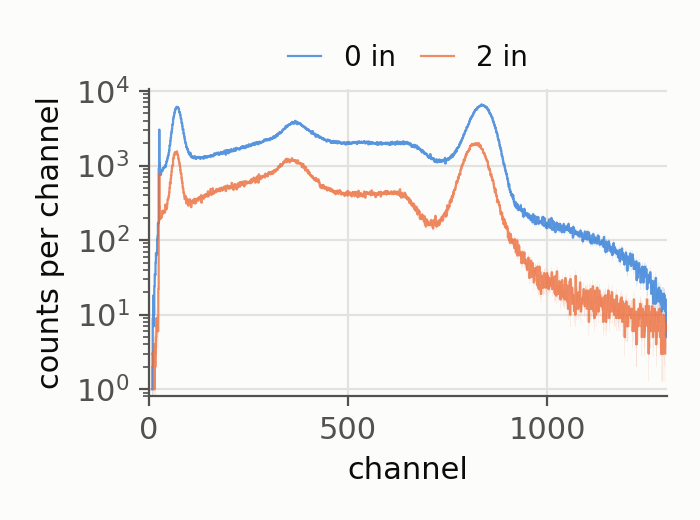
\includegraphics[width=\linewidth]{F3_raw_NaI2x2_WC.png}\caption{2''$\times$2'' NaI(Tl)}\end{subfigure}\hfill
\begin{subfigure}{0.47\textwidth}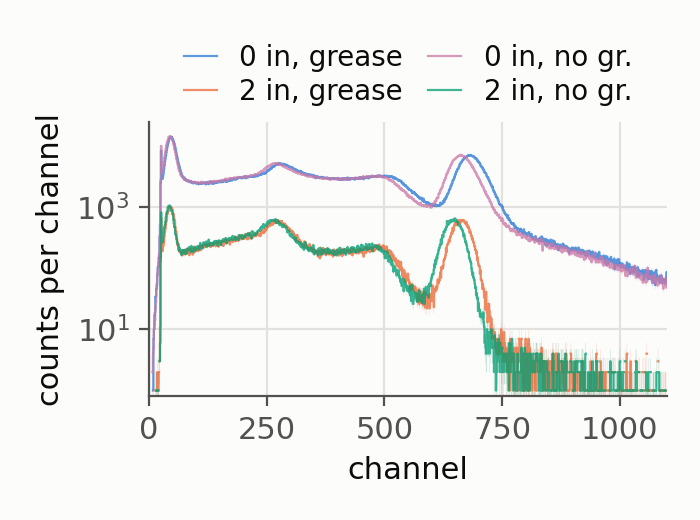
\includegraphics[width=\linewidth]{F3_raw_NaI1x1_WC.png}\caption{1''$\times$1'' NaI(Tl)}\end{subfigure}
\begin{subfigure}{0.47\textwidth}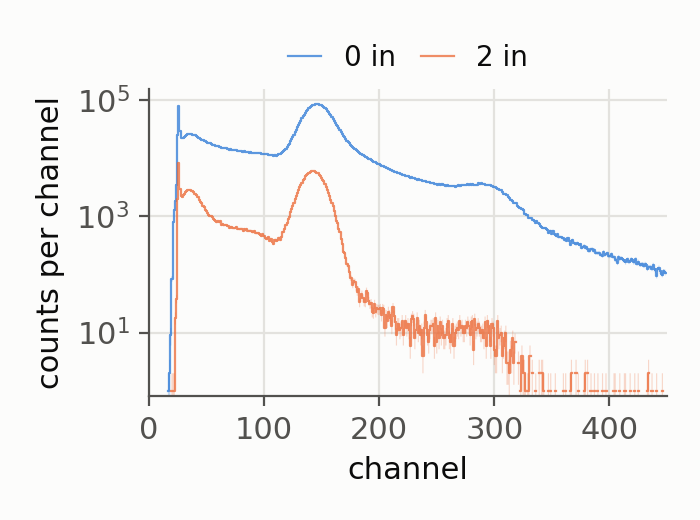
\includegraphics[width=\linewidth]{F3_raw_BGO_WC.png}\caption{BGO}\end{subfigure}\hfill
\begin{subfigure}{0.47\textwidth}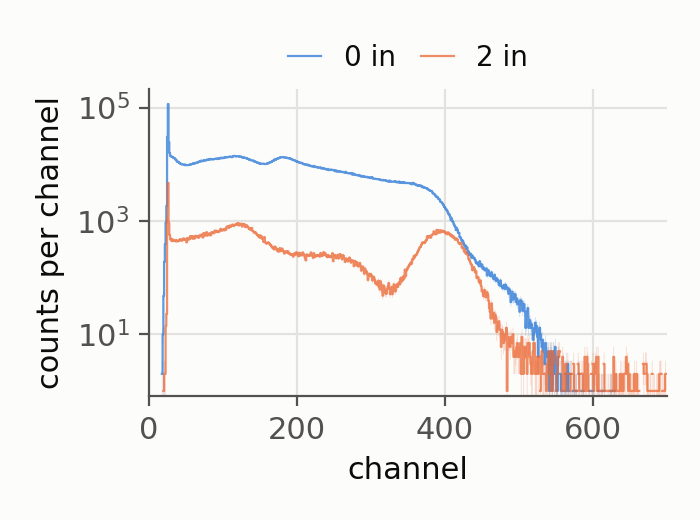
\includegraphics[width=\linewidth]{F3_raw_CsI_WC.png}\caption{CsI(Tl)}\end{subfigure}
\caption{Raw 2-min Cs-137 spectra at 0 and 2~in, log scale. The shaded band is $\pm1\sigma = \pm\sqrt{N}$ and is mostly narrower than the line. The $x$-range differs between panels.}
\label{fig:raw}
\end{figure}

\begin{figure}[!htbp]
\centering
\begin{subfigure}{0.49\textwidth}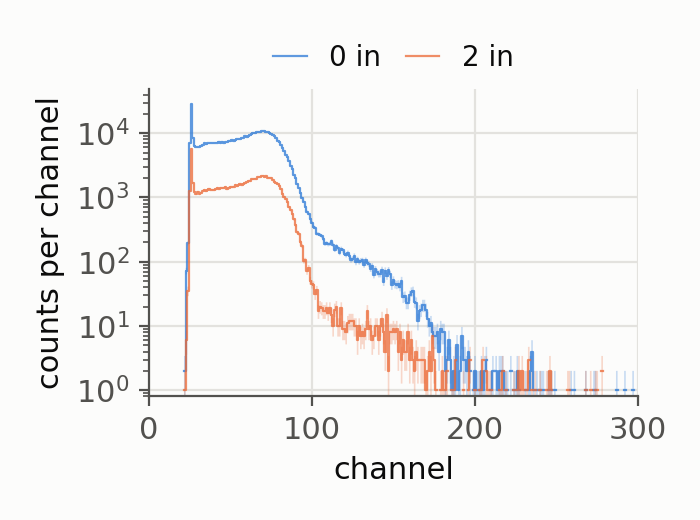
\includegraphics[width=\linewidth]{F3_raw_EJ200_WC.png}\caption{EJ-200, raw}\end{subfigure}\hfill
\begin{subfigure}{0.49\textwidth}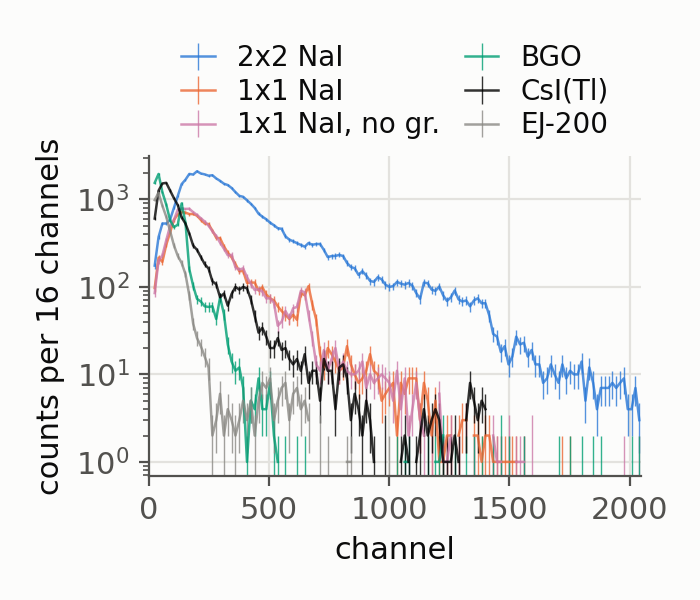
\includegraphics[width=\linewidth]{F4_backgrounds.png}\caption{Backgrounds, 240~s}\end{subfigure}
\caption{(a) Raw 2-min Cs-137 spectra of EJ-200, as in Fig.~\ref{fig:raw}. (b) The six background spectra in 16-channel bins with $\sqrt{N}$ error bars.}
\label{fig:raw2}
\end{figure}

\section{Analysis of Data}
\label{sec:analysis}

Uncertainties are propagated in quadrature from $\sigma_N = \sqrt{N}$.

\subsection{Tube Gain and Applied Voltage}
\label{subsec:an_hv}

The statistical uncertainty of a peak centroid is \cite{knoll}
\begin{equation}
\sigma_c = \frac{\text{FWHM}/2.35}{\sqrt{A}},
\label{eq:sigc}
\end{equation}
with $A$ the peak area. For the HV scan we use the FWHM and gross ROI area that MAESTRO reported at each point. To get the gain-voltage relation we fit a straight line to $\ln(\text{centroid})$ vs $\ln(\text{HV})$ by least squares over 600--1000~V. The slope is the exponent in PMT gain $\propto V^{\beta N}$ \cite{knoll}. We left out 1050--1150~V, where the centroid no longer increases.

\begin{samplecalc}{Centroid uncertainty at 1000 V (FWHM = 14.27 ch, $A$ = 3169)}
\begin{align*}
\sigma_c = \frac{14.27/2.35}{\sqrt{3169}} = \frac{6.07}{56.3} = 0.11\ \text{channels}
\end{align*}
\end{samplecalc}

The fitted slope is $5.91 \pm 0.14$ (uncertainty from the scatter of the points about the line). Figure~\ref{fig:hv} shows the centroid on linear and log-log axes.

\begin{figure}[!htbp]
\centering
\begin{subfigure}{0.49\textwidth}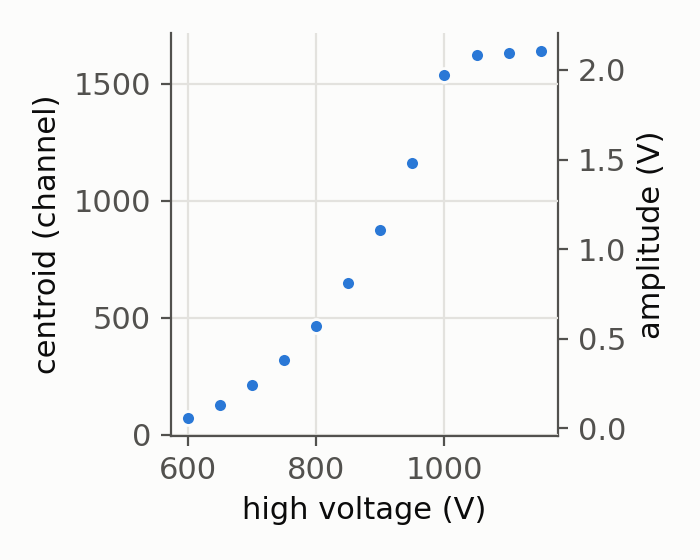
\includegraphics[width=\linewidth]{F1_hv_centroid.png}\caption{Linear axes}\end{subfigure}\hfill
\begin{subfigure}{0.49\textwidth}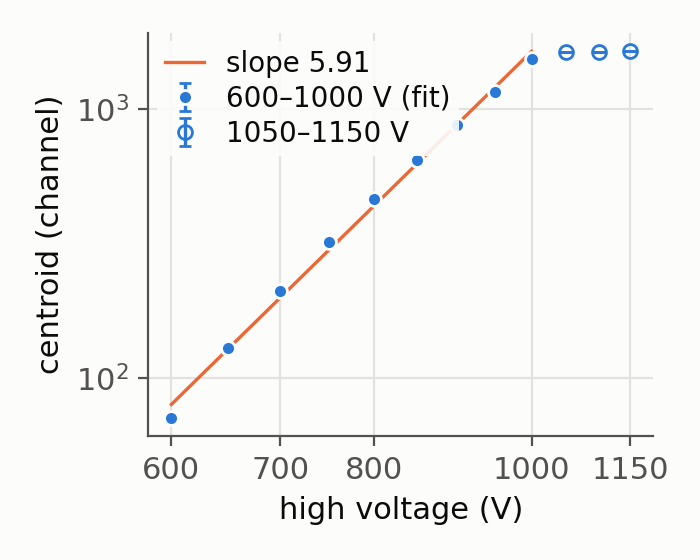
\includegraphics[width=\linewidth]{F2_hv_centroid_loglog.png}\caption{Log-log axes}\end{subfigure}
\caption{Cs-137 photopeak centroid vs HV, 2''$\times$2'' NaI(Tl). (a) Right axis: amplitude from Eq.~\ref{eq:mcacal}. (b) Line: least-squares fit to 600--1000~V (filled points), slope 5.91. Hollow points: 1050--1150~V, not fitted. Error bars (Eq.~\ref{eq:sigc}) are smaller than the markers.}
\label{fig:hv}
\end{figure}

% PARTNER: discuss the slope (PMT gain vs V) and why the centroid stops increasing above 1000 V.

\subsection{Extracting Net Peak Counts}
\label{subsec:an_net}

\textbf{Net spectrum.} The background was counted for 240~s and each source for 120~s, so we subtract background count rates and convert back to counts, channel by channel:
\begin{equation}
N_{\text{net},i} = \left(\frac{N_{s,i}}{t_s} - \frac{N_{b,i}}{t_b}\right) t_s, \qquad
\sigma_{\text{net},i}^2 = N_{s,i} + \left(\frac{t_s}{t_b}\right)^2 N_{b,i},
\label{eq:net}
\end{equation}
with live times $t_s = 120$~s and $t_b = 240$~s. The net total counts are the sum of $N_{\text{net},i}$ over all channels.

\textbf{Continuum under the photopeak.} The photopeak sits on the Compton continuum. Following Knoll, we fit a straight line to the channels on either side of the peak and subtract it channel by channel \cite{knoll}. The ROI runs from $L$ to $R$, centered on the centroid with a half-width of 1.5~FWHM. $B_L$ and $B_R$ are the mean net counts of the 3 channels just outside each edge. The line is $B_i = B_L + (B_R - B_L)(i - L)/(R - L)$ and the net photopeak counts are
\begin{equation}
A = \sum_{i=L}^{R} \left(N_{\text{net},i} - B_i\right) = \sum_{i=L}^{R} N_{\text{net},i} - n\,\frac{B_L + B_R}{2}, \qquad
\sigma_A^2 = \sum_{i=L}^{R} \sigma_{\text{net},i}^2 + \left(\frac{n}{2}\right)^2 \left(\sigma_{B_L}^2 + \sigma_{B_R}^2\right),
\label{eq:area}
\end{equation}
with $n = R - L + 1$ and $\sigma_{B}^2$ the summed variance of the 3 channels divided by 9. Since the ROI depends on the FWHM, we repeated the steps until the centroid and FWHM stopped changing.

\textbf{Centroid, FWHM and resolution.} The centroid is the count-weighted mean channel of the continuum-subtracted peak, $H_0 = \sum i\,(N_{\text{net},i} - B_i)/A$, with uncertainty from Eq.~\ref{eq:sigc}. The FWHM is the full width of the peak at half its maximum height. We take the maximum $Y$ as the mean of the 3 highest channels of the continuum-subtracted peak and find the two channels where the peak crosses $Y/2$ by linear interpolation between neighbouring channels. The uncertainty of each crossing is the counting uncertainty there divided by the local slope. The resolution follows from Eq.~\ref{eq:resolution}. It is the width of the peak relative to its position, so a smaller $R$ means the detector can separate two closer $\gamma$-ray energies \cite{knoll}. Where we also read the FWHM from MAESTRO in the lab, our values are 0.4 to 4.1 channels larger.

\begin{samplecalc}{Net counts in one channel: 2''$\times$2'' NaI(Tl), 2 in, channel 819}
\begin{align*}
N_{\text{net}} &= \left(\frac{1899}{120\ \text{s}} - \frac{10}{240\ \text{s}}\right)(120\ \text{s}) = 1899 - 5 = 1894, &
\sigma &= \sqrt{1899 + 0.5^2 \cdot 10} = 43.6
\end{align*}
\end{samplecalc}

\begin{samplecalc}{Net photopeak counts: 2''$\times$2'' NaI(Tl), 2 in (ROI channels 723--915, $n = 193$)}
\begin{align*}
\textstyle\sum N_{\text{net},i} &= 149{,}997, \qquad B_L = 148.7, \qquad B_R = 87.3\\
A &= 149{,}997 - 193\,\frac{148.7 + 87.3}{2} = 149{,}997 - 22{,}774 = 127{,}222\\
\sigma_A &= \sqrt{151{,}727 + (96.5)^2(54.1 + 30.8)} = \sqrt{941{,}687} = 970
\end{align*}
\end{samplecalc}

\begin{samplecalc}{FWHM and resolution: 2''$\times$2'' NaI(Tl), 2 in}
\begin{align*}
Y &= 1806, \quad \text{half-maximum crossings at channels } 786.9 \text{ and } 851.0\\
\text{FWHM} &= 851.0 - 786.9 = 64.1 \pm 0.6\ \text{channels}, \qquad
\sigma_{H_0} = \frac{64.1/2.35}{\sqrt{127{,}222}} = 0.08\\
R &= \frac{64.1}{818.7} = 7.82\%, \qquad
\sigma_R = R\sqrt{\left(\frac{0.63}{64.1}\right)^2 + \left(\frac{0.08}{818.7}\right)^2} = 0.08\%
\end{align*}
\end{samplecalc}

To check the ROI width we repeated the net-area calculation with half-widths of 1.0 and 2.0~FWHM. With 2.0~FWHM the net counts changed by 1.4 to 5.8\% for NaI(Tl) and BGO and by 17.7\% for CsI(Tl) at 2~in. With 1.0~FWHM they were 8 to 20\% lower for all crystals.

% PARTNER: is the net-area method reasonable? (manual question 1; use the ROI check above)

Table~\ref{tab:peaks} lists the results and Figure~\ref{fig:net} shows the net spectra. The 0~in CsI(Tl) net spectrum has no separate photopeak, only a shoulder near channel 380 (Fig.~\ref{fig:net}d), so we give no photopeak values for it. EJ-200 has no photopeak at either distance (Fig.~\ref{fig:labeled}a). Its Compton edge, taken where the spectrum falls halfway from its maximum to the minimum above it, is at channel 83.7 (0~in) and 83.8 (2~in).

\begin{table}[!htbp]
\centering\footnotesize\setlength{\tabcolsep}{3pt}
\resizebox{\textwidth}{!}{%
\begin{tabular}{lcccccc}
\toprule
\textbf{Crystal} & \textbf{Dist.} & \textbf{Centroid $H_0$ (ch)} & \textbf{FWHM (ch)} & \textbf{Net photopeak} & \textbf{$R$ (\%)} & \textbf{Net total} \\
\midrule
2''$\times$2'' NaI(Tl) & 0 in & 833.4 $\pm$ 0.04 & 63.6 $\pm$ 0.6 & 398524 $\pm$ 2209 & 7.63 $\pm$ 0.07 & 2053010 $\pm$ 1445 \\
 & 2 in & 818.7 $\pm$ 0.08 & 64.1 $\pm$ 0.6 & 127222 $\pm$ 970 & 7.82 $\pm$ 0.08 & 521320 $\pm$ 746 \\
1''$\times$1'' NaI(Tl) & 0 in & 686.0 $\pm$ 0.04 & 57.0 $\pm$ 0.4 & 379490 $\pm$ 2138 & 8.31 $\pm$ 0.05 & 2539756 $\pm$ 1596 \\
 & 2 in & 662.7 $\pm$ 0.11 & 46.6 $\pm$ 1.4 & 29800 $\pm$ 294 & 7.03 $\pm$ 0.22 & 176708 $\pm$ 431 \\
1''$\times$1'' NaI(Tl), no gr. & 0 in & 666.7 $\pm$ 0.04 & 56.2 $\pm$ 0.6 & 375235 $\pm$ 2105 & 8.43 $\pm$ 0.09 & 2496871 $\pm$ 1583 \\
 & 2 in & 646.9 $\pm$ 0.11 & 45.4 $\pm$ 0.6 & 29680 $\pm$ 313 & 7.01 $\pm$ 0.09 & 179706 $\pm$ 434 \\
BGO & 0 in & 147.4 $\pm$ 0.01 & 27.0 $\pm$ 0.1 & 2149687 $\pm$ 3863 & 18.34 $\pm$ 0.06 & 5076846 $\pm$ 2255 \\
 & 2 in & 142.9 $\pm$ 0.03 & 23.7 $\pm$ 0.3 & 141322 $\pm$ 603 & 16.58 $\pm$ 0.19 & 255834 $\pm$ 513 \\
CsI(Tl) & 0 in & -- & -- & -- & -- & 3489858 $\pm$ 1871 \\
 & 2 in & 396.9 $\pm$ 0.13 & 58.0 $\pm$ 0.9 & 35440 $\pm$ 519 & 14.60 $\pm$ 0.23 & 160960 $\pm$ 413 \\
EJ-200 & 0 in & -- & -- & -- & -- & 533586 $\pm$ 733 \\
 & 2 in & -- & -- & -- & -- & 101342 $\pm$ 324 \\
\bottomrule
\end{tabular}%
}
\caption{Photopeak results from the background-subtracted spectra (Eqs.~\ref{eq:net}--\ref{eq:area}, \ref{eq:resolution} and \ref{eq:sigc}). ``Net total'' is the net count summed over all channels. --: no photopeak. All crystals are 1''$\times$1'' and coupled with grease unless noted.}
\label{tab:peaks}
\end{table}

\begin{figure}[!htbp]
\centering
\begin{subfigure}{0.49\textwidth}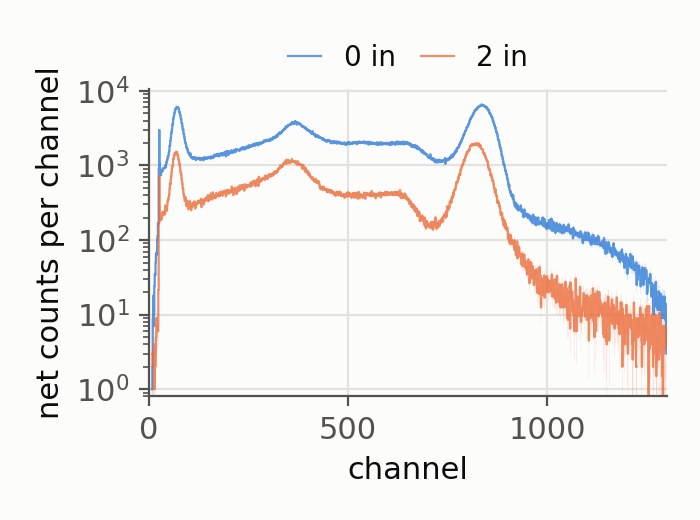
\includegraphics[width=\linewidth]{F5_net_NaI2x2_WC.png}\caption{2''$\times$2'' NaI(Tl)}\end{subfigure}\hfill
\begin{subfigure}{0.49\textwidth}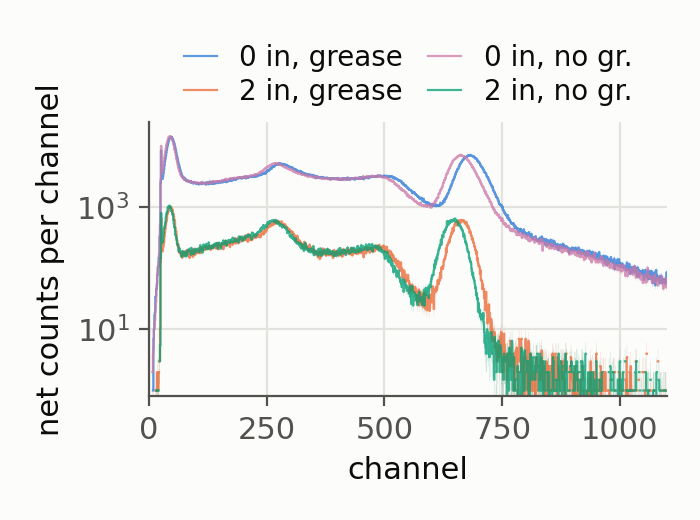
\includegraphics[width=\linewidth]{F5_net_NaI1x1_WC.png}\caption{1''$\times$1'' NaI(Tl)}\end{subfigure}
\begin{subfigure}{0.49\textwidth}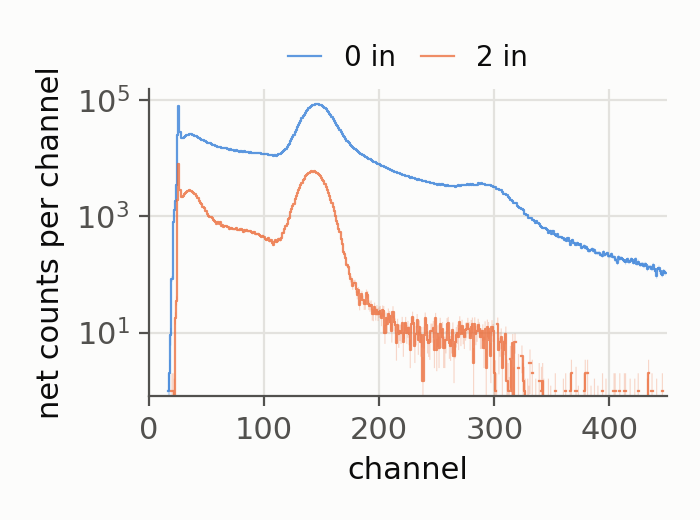
\includegraphics[width=\linewidth]{F5_net_BGO_WC.png}\caption{BGO}\end{subfigure}\hfill
\begin{subfigure}{0.49\textwidth}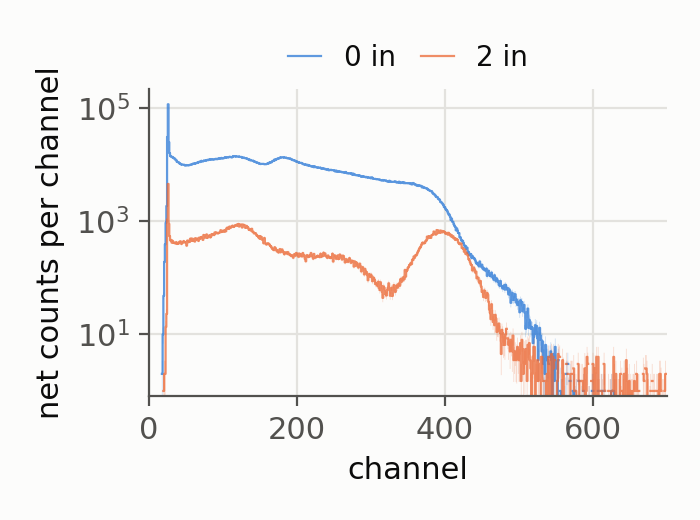
\includegraphics[width=\linewidth]{F5_net_CsI_WC.png}\caption{CsI(Tl)}\end{subfigure}
\caption{Background-subtracted spectra (Eq.~\ref{eq:net}), log scale. The shaded band is $\pm1\sigma_{\text{net}}$. Channels with net counts $\le 0$ are not drawn on the log axis.}
\label{fig:net}
\end{figure}

\textbf{Spectrum features.} We label the features of the 2''$\times$2'' NaI(Tl) spectrum at 2~in (Fig.~\ref{fig:labeled}b). To place the expected energies we assume channel is linear in energy and use two points: the Lab 2 zero (channel 27.6 at 0~V, Eq.~\ref{eq:mcacal}) and the photopeak at 662~keV \cite{knoll},
\begin{equation}
\text{channel} = 27.6 + E\,\frac{H_0 - 27.6}{662\ \text{keV}}.
\label{eq:ecal}
\end{equation}
The expected energies are the Compton edge at 478~keV (Eq.~\ref{eq:compton_edge}), the backscatter peak at 184~keV and the Ba K X-rays at about 32~keV \cite{knoll}. In the spectrum we find the X-ray and backscatter peaks as local maxima of the net spectrum (9-channel running mean), and the Compton edge as the channel where the spectrum (15-channel running mean) falls halfway from its shoulder (channel 619) to the minimum above it (channel 706).

\begin{figure}[!htbp]
\centering
\begin{subfigure}{0.49\textwidth}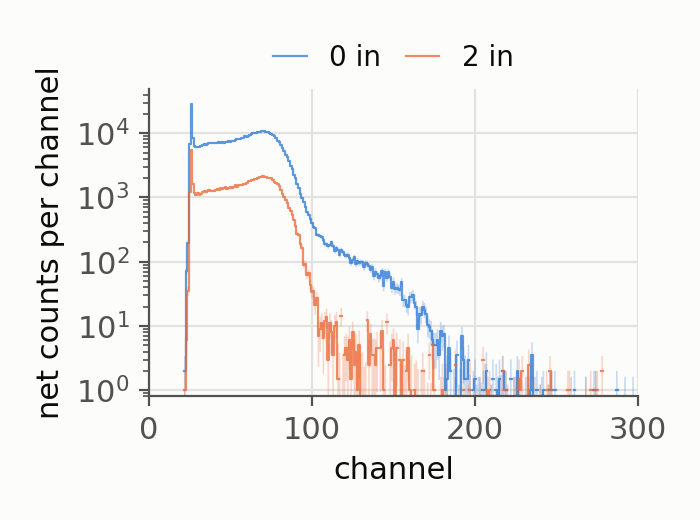
\includegraphics[width=\linewidth]{F5_net_EJ200_WC.png}\caption{EJ-200, net}\label{fig:netej}\end{subfigure}\hfill
\begin{subfigure}{0.49\textwidth}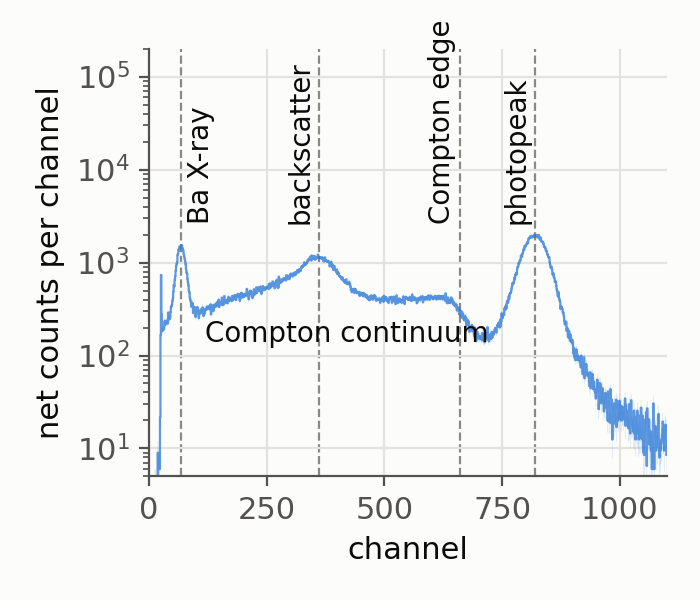
\includegraphics[width=\linewidth]{F6_labeled_NaI2x2.png}\caption{2''$\times$2'' NaI(Tl), 2 in, labeled}\label{fig:labeledb}\end{subfigure}
\caption{(a) Background-subtracted EJ-200 spectra, as in Fig.~\ref{fig:net}. (b) Net spectrum of the 2''$\times$2'' NaI(Tl), source at 2~in, shaded $\pm1\sigma$. Dashed lines at the measured features: Ba K X-ray at channel 68 (33.8~keV by Eq.~\ref{eq:ecal}), backscatter maximum at channel 361 (279~keV), Compton edge at channel 661 (530~keV) and photopeak centroid at $818.7 \pm 0.08$ with $127{,}222 \pm 970$ net counts (Table~\ref{tab:peaks}). Expected positions from Eq.~\ref{eq:ecal}: X-ray channel 66, backscatter 248, Compton edge 598.}
\label{fig:labeled}
\end{figure}

% PARTNER: describe the features (manual question 2) and compare the crystals (manual question 3).

\FloatBarrier

\section{Conclusions}
\label{sec:conclusions}



\bibliography{references}

\appendix
\section{}
\label{app:}



\end{document}
